\refstepcounter{section}
\section*{Lecture 06: Correlations and Fluctuations}
\addcontentsline{toc}{section}{Lecture 06: Correlations and Fluctuations}
In here, we discuss a bit about an important quantity, \textit{the correlation function}, which is an important quantity to look at while studying phase transition. Recall from Eq. \eqref{eqn:density1} that the density was given by a sum over delta functions. We define the \textit{density-density correlation function} (or simply the correlation function) as,
$$\SG(\vb{r},\vb{r}') = \Big\langle [n(\vb{r})-\avg{n(\vb{r})}][n(\vb{r}')-\avg{n(\vb{r}')}]\Big\rangle = \avg{n(\vb{r})n(\vb{r}')} -\avg{n(\vb{r})}\avg{n(\vb{r}')}$$
where $n(\vb{r})-\avg{n(\vb{r})}$ denotes the fluctuation of the density from its average value and $\avg{\cdot}$ represent the \textit{thermal (ensemble) average}, using the distribution. For translationally invariant system, we have $\SG(\vb{r}, \vb{r}') \equiv \SG(\vb{r}-\vb{r}')$ and also, $n(\vb{r})=n(\vb{r}')$. Then the above equation can also be written as,
$$\SG(\vb{r}-\vb{r}') = \avg{n(\vb{r})n(\vb{r}')}-n^2$$
where $\avg{n(\vb{r})}=n$. As $\abs{\vb{r}-\vb{r}'}\to \infty$, that is, the distance between two particles become very large, we do expect them to be independent and no longer `correlated'. Thus, $\SG(\vb{r}-\vb{r}')\to 0$ as $\abs{\vb{r}-\vb{r}'}\to \infty$.\\[0.2cm]
The correlation function kind of quantifies the fluctuations in the density. Earlier, we saw that the isothermal compressibility also characterises the number fluctuations. Then, these two must be related on some level. To see this, we note that 
\begin{align*}
    \Big\langle (N-\avg{N})^2 \Big\rangle &= \Big\langle \int \dd^3r\ \qty{n(\vb{r}-\avg{n(\vb{r})})}\int \dd^3r'\ \qty{n(\vb{r}'-\avg{n(\vb{r}')})} \Big\rangle\\
    &= \int \dd^3r\dd^3r'\ \Big\langle\qty{n(\vb{r}-\avg{n(\vb{r})})}\qty{n(\vb{r}'-\avg{n(\vb{r}')})} \Big\rangle = \int  \int \dd^3r\dd^3r'\ \SG(\vb{r}-\vb{r}')
\end{align*}
Introducing the variables $\vb{r}'' = \vb{r}-\vb{r}'$ and $\vb{R}= \vb{r}+\vb{r}'$, the integral changes accordingly.
$$\Big\langle (N-\avg{N})^2 \Big\rangle = \int \dd^3 R \int \dd^3 r'' \SG(r'')  = V\int \dd^3r'' \SG(r'')$$
The number fluctuation can also be written as,
$$\Big\langle (N-\avg{N})^2 \Big\rangle = \frac{\avg{N}^2\kb T}{V}\SK\tund{T} = \avg{N}n\kb T \SK\tund{T}$$
Consider an ideal gas, with $PV = N\kb T$ which gives us, 
$$\qty(\pdv{P}{V})_{T} = -\frac{N\kb T}{V^2}\implies  \tensor*{\SK}{_{\text{\tiny T}} ^\circ} = -\frac{1}{V}\qty(\pdv{V}{P}) = \frac{V}{N\kb T} =\frac{1}{n\kb T}$$
Using this, we can write the dimensionless compressiblity as,
\begin{align*}
   \qty( \frac{\SK\tund{T}}{\tensor*{\SK}{_{\text{\tiny T}} ^\circ}} )= \frac{\avg{(N-\avg{N})^2}}{\avg{N}} = \frac{V\int \dd^3 r\ \SG(r)}{\avg{N}} = \frac{1}{n}\int \dd^3 r\ \SG(r)
\end{align*}
The above is a very simple example of the \textit{fluctuation-dissipation theorem} which relates the correlation to the linear response of the system (compressibility, in our case).\\[0.2cm]
Since the isothermal compressibility diverges at $T_c$, the integral also diverges and this implies that the correlation function also becomes long ranged. The correlation length $\xi$ (the characteristic length scale after which $\SG(\vb{r})$ decays) becomes as large as the wavelength of light and the density fluctuations scatter light strongly, resulting in critical opalescence, as mentioned in sec. \ref{opal}.
\subsection{Structure Factor}
Let us now try to quantify the scattering intensity when our fluid is subjected to some radiation. Assume a \textit{quasielastic scatetring}, that is, the incoming radiation has much larger energy than the typical excitation energy of the system. Hence, the system can only absorb or emit very small amounts of energy and very small energy transfer occurs. 
\begin{figure}[H]
    \centering 
    

\tikzset{every picture/.style={line width=0.75pt}} %set default line width to 0.75pt        

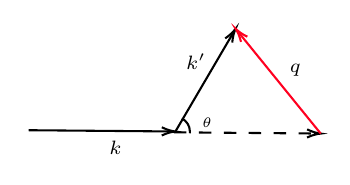
\begin{tikzpicture}[x=0.75pt,y=0.75pt,yscale=-1,xscale=1]
%uncomment if require: \path (0,583); %set diagram left start at 0, and has height of 583

%Straight Lines [id:da47989121087390596] 
\draw    (130,160) -- (198.68,160.6) ;
\draw [shift={(200.68,160.62)}, rotate = 180.5] [color={rgb, 255:red, 0; green, 0; blue, 0 }  ][line width=0.75]    (6.56,-1.97) .. controls (4.17,-0.84) and (1.99,-0.18) .. (0,0) .. controls (1.99,0.18) and (4.17,0.84) .. (6.56,1.97)   ;
%Straight Lines [id:da5560514482873335] 
\draw    (200.68,160.62) -- (228.67,112.83) ;
\draw [shift={(229.68,111.1)}, rotate = 120.36] [color={rgb, 255:red, 0; green, 0; blue, 0 }  ][line width=0.75]    (6.56,-1.97) .. controls (4.17,-0.84) and (1.99,-0.18) .. (0,0) .. controls (1.99,0.18) and (4.17,0.84) .. (6.56,1.97)   ;
%Straight Lines [id:da8910385526119278] 
\draw  [dash pattern={on 4.5pt off 4.5pt}]  (200,161) -- (268.68,161.6) ;
\draw [shift={(270.68,161.62)}, rotate = 180.5] [color={rgb, 255:red, 0; green, 0; blue, 0 }  ][line width=0.75]    (6.56,-1.97) .. controls (4.17,-0.84) and (1.99,-0.18) .. (0,0) .. controls (1.99,0.18) and (4.17,0.84) .. (6.56,1.97)   ;
%Straight Lines [id:da6496315176862661] 
\draw [color={rgb, 255:red, 255; green, 0; blue, 32 }  ,draw opacity=1 ]   (270.68,161.62) -- (230.94,112.65) ;
\draw [shift={(229.68,111.1)}, rotate = 50.94] [color={rgb, 255:red, 255; green, 0; blue, 32 }  ,draw opacity=1 ][line width=0.75]    (6.56,-1.97) .. controls (4.17,-0.84) and (1.99,-0.18) .. (0,0) .. controls (1.99,0.18) and (4.17,0.84) .. (6.56,1.97)   ;
%Shape: Arc [id:dp644522715932185] 
\draw  [draw opacity=0] (203.8,154.37) .. controls (206.09,155.52) and (207.66,157.88) .. (207.66,160.62) .. controls (207.66,160.9) and (207.64,161.19) .. (207.61,161.47) -- (200.68,160.62) -- cycle ; \draw   (203.8,154.37) .. controls (206.09,155.52) and (207.66,157.88) .. (207.66,160.62) .. controls (207.66,160.9) and (207.64,161.19) .. (207.61,161.47) ;  

% Text Node
\draw (167.34,163.71) node [anchor=north west][inner sep=0.75pt]  [font=\scriptsize]  {$\vb{k}$};
% Text Node
\draw (204.34,121.71) node [anchor=north west][inner sep=0.75pt]  [font=\scriptsize]  {$\vb{k}'$};
% Text Node
\draw (254.34,126.71) node [anchor=north west][inner sep=0.75pt]  [font=\scriptsize]  {$\vb{q}$};
% Text Node
\draw (212,152.4) node [anchor=north west][inner sep=0.75pt]  [font=\tiny]  {$\theta$};


\end{tikzpicture}

\end{figure}
\noindent
From elastic scattering, $\abs{\vb{k}}\approx \abs{\vb{k}'}$, the momentum transfer vector $\vb{q} = \vb{k}'-\vb{k}$ has a magnitude,
$$\abs{\vb{q}}=\sqrt{\abs{\vb{k}}^2+\abs{\vb{k}'}^2 -2\abs{\vb{k}}\abs{\vb{k}'}\cos\theta} \approx \sqrt{2\abs{\vb{k}}^2\qty(1-\cos\theta)} = 2\abs{\vb{k}} \sin\qty(\frac{\theta}{2})$$
Now, suppose that there are $N$ particles in the target and the \textit{scattering amplitude} for scattering from particle $i$ is $a_i(\vb{q})$. Then the total intensity of the scattered radiation is given by,
$$\mathcal{I}(q) = \avg{\abs{\sum\limits_{j=1}^N a_j(\vb{q})}^2}$$
The scattering amplitude for particles at $\vb{r}_i$ and $\vb{r}_j$ are related just by a phase factor,
$$a_j(\vb{q}) = a_i(\vb{q}) e^{-i\vb{q}\cdot (\vb{r}_j - \vb{r}_i)}$$
Using this, we can write the internsity as,
\begin{equation}
    \mathcal{I}(\vb{q}) = \avg{\abs{\sum\limits_{j=1}^N a_1(\vb{q}) e^{-i\vb{q}\cdot (\vb{r}_j - \vb{r}_1)}}^2}=\abs{a_1(\vb{q})}^2\avg{\abs{\sum\limits_{j=1}^N  e^{-i\vb{q}\cdot (\vb{r}_j - \vb{r}_1)}}^2} =\abs{a_1(\vb{q})}^2\avg{\abs{\sum\limits_{j=1}^N  e^{-i\vb{q}\cdot \vb{r}_j}}^2} 
\end{equation}
as $\abs{e^{i\vb{q}\cdot \vb{r}_1}} =1$. If no correlations exist between the particles, then $\sum\limits_j e^{-i\vb{q}\cdot(\vb{r}_j-\vb{r}_1)} = N + \sum\limits_{j\neq 1}e^{-i\vb{q}\cdot(\vb{r}_j-\vb{r}_1)}$ and $\sum\limits_{j\neq 1} \avg{e^{-i\vb{q}\cdot(\vb{r}_j-\vb{r}_1)}}\approx 0$ due to randomised phases which leads to, 
$$\tensor*{\mathcal{I}}{^\circ}(\vb{q}) = N \abs{a_1(\vb{q})}^2$$
Then we can write the dimensionless intensity as, 
\begin{align*}
    \frac{\mathcal{I}(\vb{q})}{\tensor*{\mathcal{I}}{^\circ}(\vb{q})} &=\frac{1}{N}\avg{\qty(\sum\limits_{j=1}^N  e^{i\vb{q}\cdot \vb{r}_j})\qty(\sum\limits_{i=1}^N  e^{-i\vb{q}\cdot \vb{r}_i})} =\frac{1}{N}\avg{\qty(\sum\limits_{i,j}  e^{i\vb{q}\cdot (\vb{r}_j-\vb{r}_i)})}\\
    &=\frac{1}{N}\int \dd^3r\dd^3r'\ \avg{\qty(\sum\limits_{i,j}\ddelt{\vb{r}-\vb{r}_i}\ddelt{\vb{r}'-\vb{r}_j}  e^{i\vb{q}\cdot (\vb{r}-\vb{r}')})}\\
    &=\frac{1}{N}\int \dd^3r\dd^3r'\ \avg{ e^{i\vb{q}\cdot (\vb{r}-\vb{r}')} \qty(\sum\limits_{i,j}\ddelt{\vb{r}-\vb{r}_i}\ddelt{\vb{r}'-\vb{r}_j})}\\
    &=\frac{1}{N}\int \dd^3r\dd^3r'\ e^{i\vb{q}\cdot (\vb{r}-\vb{r}')} \avg{  \qty(\sum\limits_{i}\ddelt{\vb{r}-\vb{r}_i})\qty(\sum\limits_j\ddelt{\vb{r}'-\vb{r}_j})}\\
    &=\frac{1}{N}\int \dd^3r\dd^3r'\ e^{i\vb{q}\cdot (\vb{r}-\vb{r}')} \avg{ n(\vb{r})n(\vb{r}')}\\
    &=\frac{1}{N}\int \dd^3r\dd^3r'\ e^{i\vb{q}\cdot (\vb{r}-\vb{r}')} (\SG(\vb{r}-\vb{r}')+n^2)\\
\end{align*}
Again using the same variable substitution, we obtain 
$$\frac{\mathcal{I}(\vb{q})}{\tensor*{\mathcal{I}}{^\circ}(\vb{q})} = \frac{V}{N}\int \dd^3 r\ e^{-i\vb{q}\cdot \vb{r}} \SG(\vb{r}) +\frac{V^2}{N}\int \dd^3 r \ e^{-i\vb{q}\cdot \vb{r}} = \frac{V}{N}\int \dd^3 r\ e^{-i\vb{q}\cdot \vb{r}} \SG(\vb{r}) +\frac{V^2n^2}{N}\ddelt{\vb{q}}$$
The last term contributes only when $\vb{q} =0$ which is for $\theta=0$ (forward-scattering) and is omitted in most cases. Hence, we define the structure factor $\Ss(\vb{q})$ as 
$$\Ss(\vb{q}) = \frac{n\mathcal{I}(\vb{q})}{\tensor*{\mathcal{I}}{^\circ}(\vb{q})} = \int \dd^3 r\ e^{-i\vb{q}\cdot \vb{r}} \SG(\vb{r})$$
$\Ss(\vb{q})$ is just the spatial Fourier transform of the correlation function. $\Ss(\vb{q})$ becomes extremely large as we approach the critical point, for small values of $\abs{\vb{q}}$. 